\documentclass[11pt]{article}
\marginparwidth 0.5in 
\oddsidemargin 0.25in 
\evensidemargin 0.25in 
\marginparsep 0.25in
\topmargin 0.25in 
\textwidth 6in \textheight 8 in
\usepackage{amsmath}
\usepackage{amssymb}
\usepackage{graphicx}
\usepackage[T2A]{fontenc}
\usepackage[utf8]{inputenc}
\usepackage[russian]{babel}
\begin{document}
	\begin{titlepage}
		\begin{center}
					
			\large Московский физико-технический институт
			\vspace{0.25cm}
			
			\large Бельдий Дмитрий\\
			1 курс, 773 группа
			\vfill
			
			\textsc{\LARGE Вопрос по выбору}\\[10mm]
			
			{\Huge МАЯТНИК ФУКО}
			\bigskip
			
			
		\end{center}
		
		\vfill
		
		\begin{center}
			29.12.2017
		\end{center}
	\end{titlepage}

\begin{center}
	\textbf{{\large Историческая справка}}
\end{center}
Французский физик и астроном Жан Фуко \textbf{впервые} осуществил свой эксперимент \textbf{$8$ января $1851$ года} в погребе своего дома. Для этого был использован маятник длиной 2 метра. В феврале с разрешения Доминика Франсуа Араго он повторил опыт в Парижской обсерватории, на этот раз удлинив маятник до $11$ метров. В подготовке эксперимента принимал также участие ассистент Фуко Фромент. \textbf{Первая публичная демонстрация} была осуществлена уже в марте $1851$ года в парижском Пантеоне: под куполом Пантеона он подвесил металлический \textbf{шар массой $28$ кг} с закрепленным на нём остриём на стальной проволоке \textbf{длиной $67$ м}. Крепление маятника позволяло ему свободно колебаться во всех направлениях, под точкой крепления было сделано круговое ограждение \textbf{диаметром $6$ м}, по краю ограждения была насыпана песчаная дорожка таким образом, чтобы маятник в своём движении мог при её пересечении прочерчивать на песке отметки. \textbf{Чтобы избежать бокового толчка} при пуске маятника, его отвели в сторону и привязали верёвкой, после чего верёвку пережгли. \textbf{Период колебания} маятника при такой длине подвеса составлял \textbf{$16,4$ секунды}, при каждом колебании отклонение от предыдущего пересечения песчаной дорожки составляло около $3$ мм, \textbf{за час} плоскость колебаний маятника поворачивалась более чем на \textbf{$11^{\circ}$} по часовой стрелке, то есть примерно за \textbf{$32$ часа} совершала полный оборот и возвращалась в \textbf{прежнее положение.}\\
\\
\begin{center}
	\textbf{{\large Теоретическая справка}}
\end{center}
Маятник Фуко представляет собой математический маятник.\\
Опыт с маятником Фуко показывает, что Земля (как и другие планеты Солнечной системы), является НИСО. Если бы Земля была ИСО, то на маятник действовали бы только “настоящие силы”: т.е. сила тяжести $F=mg$ и сила натяжения нити $T$, сила трения нити и сопротивление воздуха (последними двумя можно пренебречь для рассмотрения теоретической части вопроса). В таком случае плоскость колебаний маятника оставалась неподвижной в СО Земли, однако она совершает вращение вокруг оси, проходящей через нить подвеса в состоянии покоя маятника. Значит верно обратное: Земля является НИСО. Предположим, что Земля вращается в некоторой ИСО. Тогда к к “настоящим силам” добавятся еще силы инерции: центробежная и кориолисова. Движение маятника будет описываться уравнением:\\
$$m\vec{a}=m\vec{g}+2m[\vec{v}\cdot\vec{\omega}]+\vec{T}\,\,\,\,\,(1),$$
где $2m[\vec{v}\cdot\vec{\omega}]=\vec{F}_k$ - кориолисова сила, которая и поворачивает плоскость колебаний маятника.\\
Рассмотрим \underline{частный случай}: пусть маятник расположен ровно на полюсе, тогда $\vec{\omega}$ проходит вдоль оси вращения Земли, и результат очевиден в ИСО: плоскость маятника неподвижна, вращается Земля, на маятник не действуют никакие  силы инерции.\\
В общем случае будем рассматривать уравнение $(1)$ СО Земли на широте $\theta$. Разложим вектор $\vec{\omega}$ на вертикальную и горизонтальную составляющие:\\
$$\vec{\omega}=\vec{\omega}_{v}+\vec{\omega}_{g},$$
$$\vec{\omega}_{v}=\vec{\omega}\sin\theta,$$
$$\vec{\omega}_{g}=\vec{\omega}\cos\theta,$$
Разложим $\vec{\omega}_{g}$ на составляющие $\vec{\omega}_{||}$ и $\vec{\omega}_{\perp}$.\\
\begin{figure}[bh]
	\noindent\centering{
		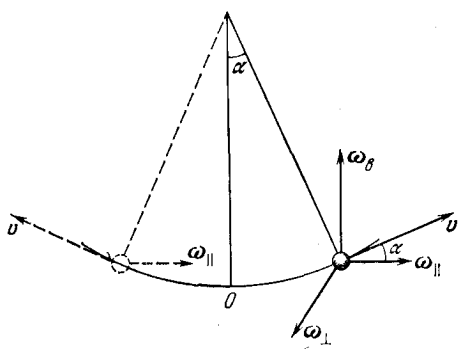
\includegraphics[width=120mm]{1.png}
	}
	\caption{Рисунок 1.}
	\label{figCurves}
\end{figure}
\\
Таким образом уравнение $(1)$ можно переписать в таком виде:
$$m\vec{a}=m\vec{g}+2m[\vec{v}\cdot\vec{\omega}_{v}]+2m[\vec{v}\cdot\vec{\omega}_{||}]+2m[\vec{v}\cdot\vec{\omega}_{\perp}]+\vec{T}\,\,\,\,\,(2).$$
Вектор $\vec{\omega}_{||}$ сонаправлен с силой $T$, поэтому влияет только на нее (с удлинением нити увеличивается период колебаний). Вектор $\vec{\omega}_{\perp}$ очень интересен тем, что он всегда сохраняет свое направление, таким образом вектор $2m[\vec{v}\cdot\vec{\omega}_{\perp}]$ перпендикулярен (за плоскость рисунка) плоскости колебаний маятника в крайних положениях, и направлена противоположно при приближении маятника к положению покоя. Значит эта составляющая вызывает только мелкие аберрации плоскости, зависящие от угла отклонения маятника, а при маленьких углах эти аберрации незначительно, значит эта составляющая на влияет на поворот плоскости маятника на большие углы. Составляющая силы Кориолиса $2m[\vec{v}\cdot\vec{\omega}_{v}]$ перпендикулярна плоскости колебаний маятника, и вызывает ее поворот. Пренебрегая $2m[\vec{v}\cdot\vec{\omega}_{\perp}]$, $2m[\vec{v}\cdot\vec{\omega}_{||}]$ и $T$,  уравнение $(2)$ приводим к такому виду:\\
$$m\vec{a}=m\vec{g}+2m[\vec{v}\cdot\vec{\omega}_{v}]\,\,\,\,\,(3).$$
Таким образом мы получили уравнение общего вида для маятника Фуко. Заменив $\vec{\omega}_{v}$ на $\omega\cdot\sin\theta$ можем решать задачи для маятника расположенного на любой широте. Для полюса $\sin(90^{\circ})=1$, т.е. эквивалентно частному случаю.\\
\\\begin{center}
	\textbf{{\large Анализ и разработка модели}}
\end{center}
$$t=\frac{2\pi}{\omega\cdot\sin\theta}=\frac{T}{\sin\theta},$$
где $t$ - время полного оборота плоскости маятника вокруг своей оси, $T$ - период вращения Земли относительно ИСО.\\
Угловая скорость вращения Земли $\omega=\frac1{240}=0,00416\, [\frac{\mathrm{deg}}{\mathrm{sec}}]$\\
В опыте Фуко в использовался груз массой $28$кг и подвес длинной $67$м для того, чтоб маятник за сутки совершил полный оборот без существенной потери амплитуды. Период колебания такого маятника составляет $16,4$с.\\
Проекция центра шара (конца подвеса) на плоскость, которая касается Земли в проекции центра шара на поверхность Земли (назовем ее плоскостью платформы, над которой маятник совершает колебания), описывает траекторию, подобную лепесткам цветка.\\
\\
Широта Парижа $= 48.5^\circ$.\\
В опыте Фуко $t=\frac{86400\,\mathrm{c}}{\sin(48.5^{\circ})}=115360\,\mathrm{c}=32.044$ часа, что равно данным, полученным  опыте.\\
За час маятник совершает $\frac{3600}{16.4} = 219.51$ колебание, поворачиваясь на $11.02^{\circ}$, т.е. каждое колебание он поворачивается на $0.05^{\circ}$. В опыте сказано, что каждое последующее колебание смещалось на $3$мм по окружности в крайней точке. Рассчитаем угол, сжимающий дугу $3$мм окружности радиусом $3$м:
$$\alpha = \frac{1}{r} = \frac{3\,\mathrm{mm}}{3\,\mathrm{m}} = 0.001\,\mathrm{rad} = 0.057^{\circ}$$
Т.е. опыт имел погрешность $\sim12\%$.\\
\\
Угол между двумя соседними лепестками (оставленными от проекций центра шара на плоскость платформы в двух крайних положениях маятника в пределах одного колебания) можно рассчитать по формуле:
$$\alpha = 180^{\circ} - \omega\cdot t,$$
где $t$ - полупериод колебания маятника, т.е. $t=180^{\circ} - \omega\cdot2\pi\cdot\frac{\sqrt{\frac lg}}2= 180^{\circ} - \omega\cdot\pi\cdot\sqrt{\frac lg}.$\\
В опыте Фуко угол между лепестками составлял $179.943^{\circ}$.

Например, при $\omega = \frac{10\pi}{3T}$ получим замкнутую траекторию с тремя лепестками, а при $\omega = \frac{14\pi}{T}$ - с четырьмя.



При разработке использовал JavaScript ES6, ReactJS library. Исходный код опубликован в GitHub репозитории по ссылке: github.com/mityabeldii/foucault-pendulum
По состоянию на 29.12.17 модель поддерживает эмуляцию ИСО и НИСО, используемых в ходе доказательства того факта, что Земля является НИСО, и объяснения природы вращения плоскости маятника. Маятник поддерживает затухающие и незатухающие (damped button) колебания с фиксированным коэффициентом затухания $\beta = 0.05$. Изменение длины подвеса маятника и угловой скорости вращения НИСО не реализованы в виде графического интерфейса, однако эти значения можно менять в файле состояния MainReduser.js. Ко всем физическим вычислениям приведены комментарии в коде. Также реализована возможность построения графика координаты $x(t)$ центра шара от времени $t$. Платформа может вращаться, а маятник совершать колебания независимо друг от друга, таким образом на данной модели можно продемонстрировать природу гармонических затухающих и незатухающих колебаний, а также определить вектор угловой скорости.

P.S.: модель, возможно, будет доступна по ссылке mityabeldii.github.io/foucault-pendulum/, иначе - по описанию в репозитории.\\

\begin{thebibliography}{0}
	\bibitem{knuth93texbook}
	Д. В. Сивухин, ОБЩИЙ КУРС ФИЗИКИ МЕХАНИКА, 1979 г.
	\bibitem{lvovsky94latex} ru.wikipedia.org/wiki/Маятник$\_$Фуко
\end{thebibliography}
\end{document}